\documentclass[12pt]{article}
\usepackage{graphicx}
\usepackage[none]{hyphenat}
\usepackage{graphicx}
\usepackage{listings}
\usepackage[english]{babel}
\usepackage{graphicx}
\usepackage{caption} 
\usepackage{booktabs}
\usepackage{array}
\usepackage{amssymb} % for \because
\usepackage{amsmath}   % for having text in math mode
\usepackage{extarrows} % for Row operations arrows
\usepackage{listings}
\lstset{
  frame=single,
  breaklines=true
}
\usepackage{hyperref}
\usepackage{mathtools}

%Following 2 lines were added to remove the blank page at the beginning
\usepackage{atbegshi}% http://ctan.org/pkg/atbegshi
\AtBeginDocument{\AtBeginShipoutNext{\AtBeginShipoutDiscard}}


%New macro definitions
\newcommand{\mydet}[1]{\ensuremath{\begin{vmatrix}#1\end{vmatrix}}}
\providecommand{\brak}[1]{\ensuremath{\left(#1\right)}}
\providecommand{\sbrak}[1]{\ensuremath{{}\left[#1\right]}}
\providecommand{\norm}[1]{\left\lVert#1\right\rVert}
\providecommand{\abs}[1]{\left\vert#1\right\vert}
\newcommand{\solution}{\noindent \textbf{Solution: }}
\newcommand{\myvec}[1]{\ensuremath{\begin{pmatrix}#1\end{pmatrix}}}
\let\vec\mathbf


\begin{document}

\begin{center}
\title{\textbf{Convex Optimization}}
\date{\vspace{-5ex}} %Not to print date automatically
\maketitle
\end{center}
\setcounter{page}{1}

\section{12$^{th}$ Maths - Chapter 6}
This is Problem-1(i) from Exercise 6.5
\begin{enumerate}
\item Detrmine whether the function $f\brak{x} = \brak{2x-1}^2 + 3$ is convex or not. \\ 
\solution 
A single variable function $f$ is said to be convex if
\begin{align}
	\label{eq:convex_def}
        f\sbrak{\lambda a + \brak{1-\lambda}b} \leq \lambda f\brak{a} + \brak{1-\lambda}f\brak{b},
\end{align}
for $\quad 0 < \lambda < 1$.
The given function is 
\begin{align}
	\label{eq:givenFunc}
	 f\brak{x} &= \brak{2x-1}^2 + 3
\end{align}
Consider two points $a, b$ on x-axis. 
\begin{align}
	a &= 0 \\
	b &= 1.25 \\
	\lambda &= 0.45
\end{align}
Substituting above values in Equation \eqref {eq:convex_def}
\begin{align}
        f\sbrak{\lambda a + \brak{1-\lambda}b} &= f\sbrak{0.45\brak{0} + \brak{1-0.45}1.25} \\ 
	\label{eq:Inequality1}
	&= f\sbrak{0.6875} = 3.141 \\
	\lambda f\brak{a} + \brak{1-\lambda}f\brak{b} &=  0.45f\brak{0} + \brak{1-0.45}f\brak{1.25} \\
	\label{eq:Inequality2}
	&=  0.45\brak{4} + \brak{0.55}\brak{5.25}  = 4.6875\\
	\eqref{eq:convex_def} \implies 3.141 \leq 4.6875 
\end{align}
$\because$ The above inequality holds true, the given equation is convex.
The figure is as shown in Fig\ref{fig:Fig1}
\begin{figure}[!h]
	\begin{center}
		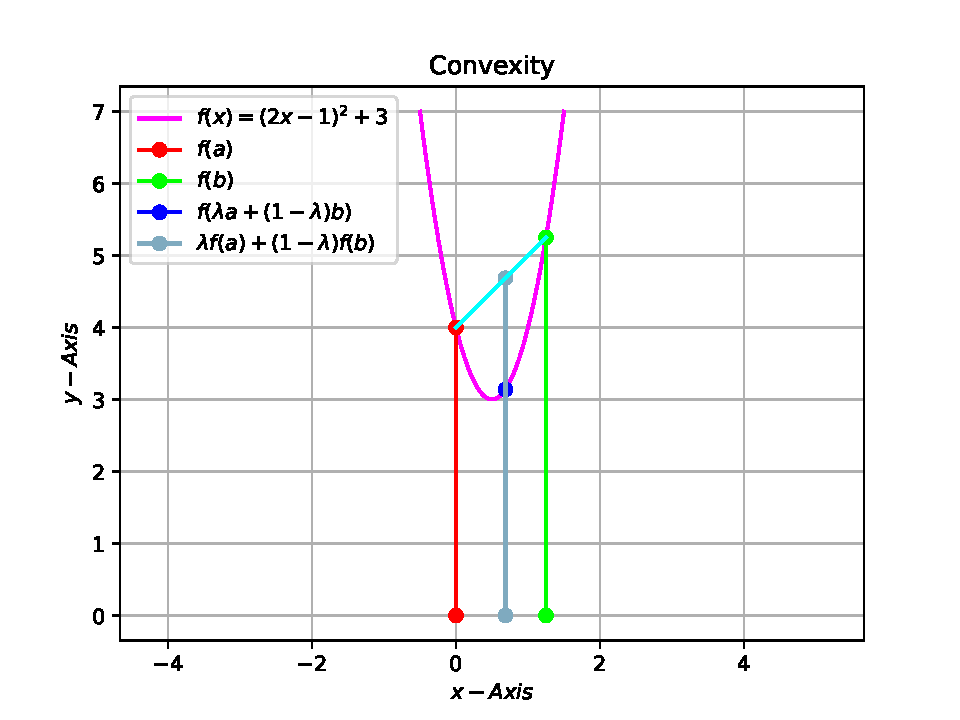
\includegraphics[width=\columnwidth]{./figs/problem1.pdf}
	\end{center}
\caption{}
\label{fig:Fig1}
\end{figure}
\end{enumerate}
\end{document}
